\chapter{Data Mining Methods}
\label{ch:mining}

This chapter introduces the data transformation method used in this dissertation.
\section{Remove invalid or missing data}
As a real-world applications of data mining, there are some invalid or missing data in the original data collection. This system should automatically remove invalid data from the raw data and replace missing values with rational information. The rule to handle data is as follows,

\clearpage
\begin{itemize}
	\item Data on holiday. One example is in figure~\ref{fg:invalid_data}, Jan 1, 2016 is New Year Day, and Dec 25, 2015 is Christmas day. There are no transactions on these two days, but in Yahoo Finance, holidays like there are still listed there. Information about Hong Kong holidays are collected from http://www.timeanddate.com/, and after downloading data from Yahoo Finance, the system would automatically remove these holiday transaction data.
	\begin{figure}[h]
		\centering
		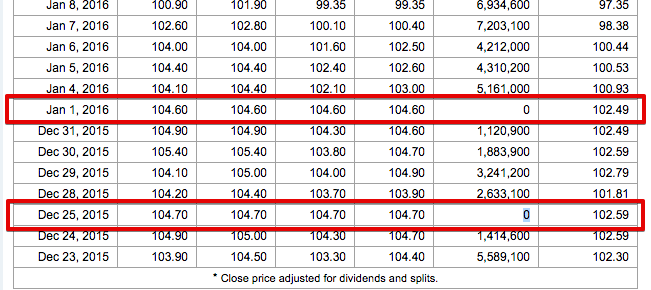
\includegraphics[width=0.9\textwidth]{invalid-data}
		\caption{Example for invalid data}
		\label{fg:invalid_data}
	\end{figure}
	\item Missing data. Like figure~\ref{fg:missing_data}, the overnight and 1-week rate is inaccessible on that day. In this case, the system would automatically use valid previous information to instead this value.
	\begin{figure}[h]
		\centering
		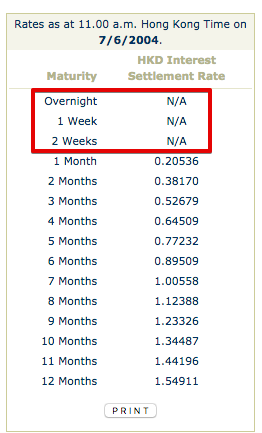
\includegraphics[width=0.6\textwidth]{missingdata}
		\caption{Example for missing data}
		\label{fg:missing_data}
	\end{figure}
	\clearpage
	\item Time difference. This is a big issue when the system queries some data based on different time zone from Hong Kong Time (HKT, GMT+8), e.g. New York time (GMT -4), which is 12 hours behind HKT. Obviously, at the beginning of each transaction day in Hong Kong, it is impossible to get the same day information in NY. Thus, the date of data at NYT should be one day prior to that in HKT.
\end{itemize}


The above are data cleaning rules in this system, and after the above processing, clean data would do the following step, normalization.


\section{Data Normalization}

The main objective of data normalizations is to guarantee the quality of the data before it is imported to learning methods, as if using non-normalized data, the algorithm may overweight those features with larger values, or underestimate those with smaller values. Data normalization can also speed up training process because in the initial, each feature is in the same scale.\\



In this study two normalization methods are mainly used to ensure the data is in same scale.

\subsection{Min-Max Normalization\cite{4_kantardzic}}
This technique obtains distribution of values on a predefined normalized interval, for example [0, 1], or [-1, 1]. In this study, the data range is usually [-1, 1], formula used here is,



\begin{equation}
v'(i)=\frac{2\times v(i)- (max(v(i))+min(v(i)))}{max(v(i))-min(v(i))}
\end{equation}

The problem of using min-max normalization method in stock price prediction is that the minimum and maximum values of out-of-sample data remain unknown at start. \\


To solve this problem, the maximum and minimum value used in this system is the highest and lowest price over the last 5 days. It is true that if the price keeps going up or down in the time period (including the predicting day), the normalized value may larger than 1 or smaller than -1.


\subsection{Standard Deviation Normalization\cite{4_kantardzic}}


Standard deviation normalization often works well in scale measures but transforms the original data into a different form, i.e., this type of normalization changes the pattern of original data. In this study, the equation of Standard Deviation is as below,


\begin{equation}
v'(i)=\frac{v(i)-mean(v)}{std(v)}
\end{equation}

This normalization method shares same problem with min-max, the mean average and standard deviation of out-of-sample data is unknown. \\



To avoid this problem, in this experiment, standard deviation normalization is mainly used to normalize the absolute difference value of price.
\clearpage

\subsection{Sigmoid Normalization\cite{nayak2014impact}}
This normalization method is used in the training process of Artificial Neural Network. The data value $v$ is computed through,


\begin{equation}
v'(i)=\frac{1}{1+e^{v(i)}}
\end{equation}

One advantage of this type of normalization is that no previous knowledge of data is needed. But it is not suitable to transform raw data directly as the scale of original is a little large.


\section{Principal Components Analysis}

To interpret a large dataset in a more meaningful form, it is necessary to reduce the number of variables to a few, interpretable linear combinations of the data. PCA is probably the most widely-used and well-known of the “standard” multivariate methods. PCA first invented by Pearson \cite{peason1901lines}, is a useful tool to extract relevant information from data sets, and provides a method to reduce a complex data set to a lower dimension. Practical applications confirmed that PCA is the best linear dimension-reduction technique in the mean-square-error sense.\cite{4_kantardzic}. \\

PCA takes a data matrix of n objects by p variables, which may be correlated, and summarizes it by uncorrelated axes (principal components or principal axes) that are linear combinations of the original p variables. The first k components display as much as possible of the variation among objects.

\subsection{Procedure of PCA\cite{4_kantardzic}}

Suppose that we have a random vector $\textbf{X}$.
\begin{equation}
\textbf{X} = \left(\begin{array}{c} X_1\\ X_2\\ \vdots \\X_p\end{array}\right)
\end{equation}
Our goal is to develop a new set of p axes (linear combinations of the original p axes) in the directions of greatest variability, as Figure~\ref{fg:pca_pitcure} shows. This goal is accomplished by rotating the axes.

\begin{figure}[h]
	\centering
	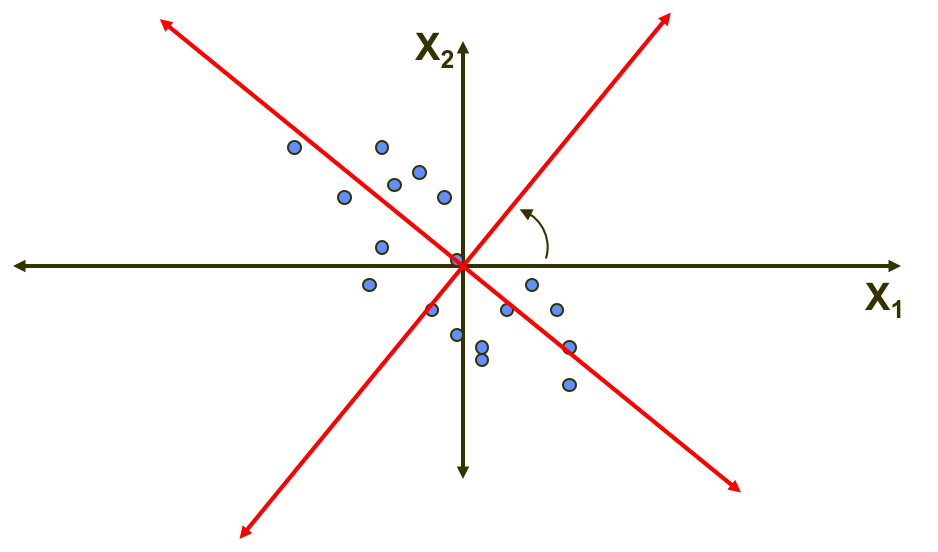
\includegraphics[width=0.6\textwidth]{pca-picture}
	\caption{Rotating the axes}
	\label{fg:pca_pitcure}
\end{figure}

Suppose our vector with covariance matrix $\Sigma$
\begin{equation}
\text{var}(\textbf{X}) = \Sigma = \left(\begin{array}{cccc}\sigma^2_1 & \sigma_{12} & \dots &\sigma_{1p}\\ \sigma_{21} & \sigma^2_2 & \dots &\sigma_{2p}\\  \vdots & \vdots & \ddots & \vdots \\ \sigma_{p1} & \sigma_{p2} & \dots & \sigma^2_p\end{array}\right)
\end{equation}

And eigenvalues $ \lambda_1 \ge \lambda_2 \ge \dots \ge \lambda_p $ \\

We have to construct p linear combinations

\begin{equation}
\text{var}(\textbf{X}) = \Sigma = \left(\begin{array}{cccc}\sigma^2_1 & \sigma_{12} & \dots &\sigma_{1p}\\ \sigma_{21} & \sigma^2_2 & \dots &\sigma_{2p}\\  \vdots & \vdots & \ddots & \vdots \\ \sigma_{p1} & \sigma_{p2} & \dots & \sigma^2_p\end{array}\right)
\end{equation}

Note that $ Y_i $ is a function of our random data, and is also stochastic. Therefore it has a population variance
\begin{equation}
\begin{array}{lll} 
Y_1 & = & e_{11}X_1 + e_{12}X_2 + \dots + e_{1p}X_p \\ Y_2 & = & e_{21}X_1 + e_{22}X_2 + \dots + e_{2p}X_p \\ & & \vdots \\ Y_p & = & e_{p1}X_1 + e_{p2}X_2 + \dots +e_{pp}X_p
\end{array}
\end{equation}

Moreover, $ Y_i $ and $ Y_j $ have a population covariance

\begin{equation}
\text{cov}(Y_i, Y_j) = \sum_{k=1}^{p}\sum_{l=1}^{p}e_{ik}e_{jl}\sigma_{kl} = \mathbf{e}'_i\Sigma\mathbf{e}_j
\end{equation}

The coefficients $ e_{ij} $ are collected into the vector

\begin{equation}
\mathbf{e}_i = \left(\begin{array}{c} e_{i1}\\ e_{i2}\\ \vdots \\ e_{ip}\end{array}\right)
\end{equation}

The principal components are those uncorrelated linear combinations $ Y_1,\dots,Y_p $ whose variances are as large as possible. 
Then the first principal component is the linear combination of maximum variance, i.e.
\begin{equation}
\text{var}(Y_1) = \sum_{k=1}^{p}\sum_{l=1}^{p}e_{1k}e_{1l}\sigma_{kl} = \mathbf{e}'_1\Sigma\mathbf{e}_1
\end{equation}

subject to the constraint that
\begin{equation}
\mathbf{e}'_1\mathbf{e}_1 = \sum_{j=1}^{p}e^2_{1j} = 1
\end{equation}

The second principal component is the linear combination of maximum variance that is uncorrelated with the first principal component. Which means that we should select $ e_{21}, e_{22}, \dots, e_{2p} $ that maximizes the variance of this new component

\begin{equation}
\text{var}(Y_2) = \sum_{k=1}^{p}\sum_{l=1}^{p}e_{2k}e_{2l}\sigma_{kl} = \mathbf{e}'_2\Sigma\mathbf{e}_2
\end{equation}
subject to the constraint that the sums of squared coefficients add up to one,
\begin{equation}
\mathbf{e}'_2\mathbf{e}_2 = \sum_{j=1}^{p}e^2_{2j} = 1
\end{equation}
along with the additional constraint that these two components will be uncorrelated with one another.
\begin{equation}
\text{cov}(Y_1, Y_2) = \sum_{k=1}^{p}\sum_{l=1}^{p}e_{1k}e_{2l}\sigma_{kl} = \mathbf{e}'_1\Sigma\mathbf{e}_2 = 0
\end{equation}
All the subsequent principal components are linear combinations that account for as much of the remaining variation as possible with the constraint that not correlated with other principal components.\\
For the $ i^{th} $ principal component $ Y_i $ we should select $ e_{i1}, e_{i2}, \dots, e_{ip} $ that maximizes the variance of this new component

\begin{equation}
\text{var}(Y_i) = \sum_{k=1}^{p}\sum_{l=1}^{p}e_{ik}e_{il}\sigma_{kl} = \mathbf{e}'_i\Sigma\mathbf{e}_i
\end{equation}

subject to the constraint that sums of squared coefficients add up to one, along with the additional constraint that this new component will be uncorrelated with all the previously defined components.

\begin{gather*}
\mathbf{e}'_i\mathbf{e}_i = \sum_{j=1}^{p}e^2_{ij} = 1\\
\text{cov}(Y_1, Y_i) = \sum_{k=1}^{p}\sum_{l=1}^{p}e_{1k}e_{il}\sigma_{kl} = \mathbf{e}'_1\Sigma\mathbf{e}_i = 0\\
\text{cov}(Y_2, Y_i) = \sum_{k=1}^{p}\sum_{l=1}^{p}e_{2k}e_{il}\sigma_{kl} = \mathbf{e}'_2\Sigma\mathbf{e}_i = 0\\
\vdots\\
\text{cov}(Y_{i-1}, Y_i) = \sum_{k=1}^{p}\sum_{l=1}^{p}e_{i-1,k}e_{il}\sigma_{kl} = \mathbf{e}'_{i-1}\Sigma\mathbf{e}_i = 0
\end{gather*}

The following figure shows the visualization before and after PCA.
\begin{figure}[h]
	\centering
	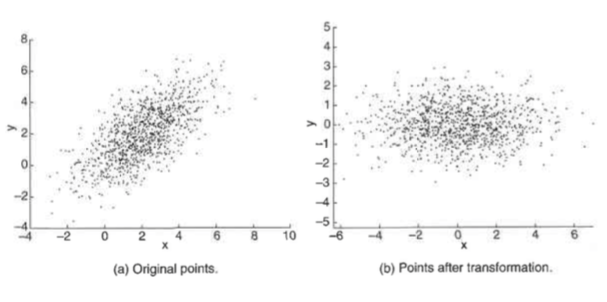
\includegraphics[width=0.8\textwidth]{pca-transform}
	\caption{Data visualization before and after PCA transformation\cite{6_tan_steinbach_kumar_2005}}
\end{figure}

\clearpage
\section{Summary}
This chapter introduces data select rule and transform methods used this this dissertation. After the above process, the output data would be clean and normalized, which is suitable for further process.
